%% OTP_CPP1_AI_Narrative.tex
%% Competitive Preference Priority 1 -- Advancing Artificial Intelligence
%% in Education (91 FR 18774). Separate attachment, NO MORE THAN 3 PAGES.
%% Up to 10 points. ED will not award points unless the application
%% clearly identifies CPP1 -- state it explicitly here and in the abstract.
\documentclass[12pt,letterpaper]{article}
\usepackage{otpgrant}

\begin{document}
\doublespacing

\begin{center}
  {\bfseries Competitive Preference Priority 1:\\
  Advancing Artificial Intelligence in Education}
\end{center}

\noindent This application addresses Competitive Preference Priority 1
under the Secretary's Supplemental Priority and Definitions on Advancing
Artificial Intelligence in Education (91 FR 18774).

\section*{AI for Students}
% Adaptive learning technologies, virtual teaching assistants, tutoring,
% data analytics supporting student progress and differentiated instruction.

As part of OTP Phase I,  we were able to integrate HaLLMos (\url{https://hallmos.com/}) chat boxes into Ximera. This allows students to answer open-ended, free-response questions and receive immediate AI-guided feedback (See Figure \ref{F:hallmos}).   
\begin{figure}[h]
  \centering
  \caption{A HaLLMos window.}
  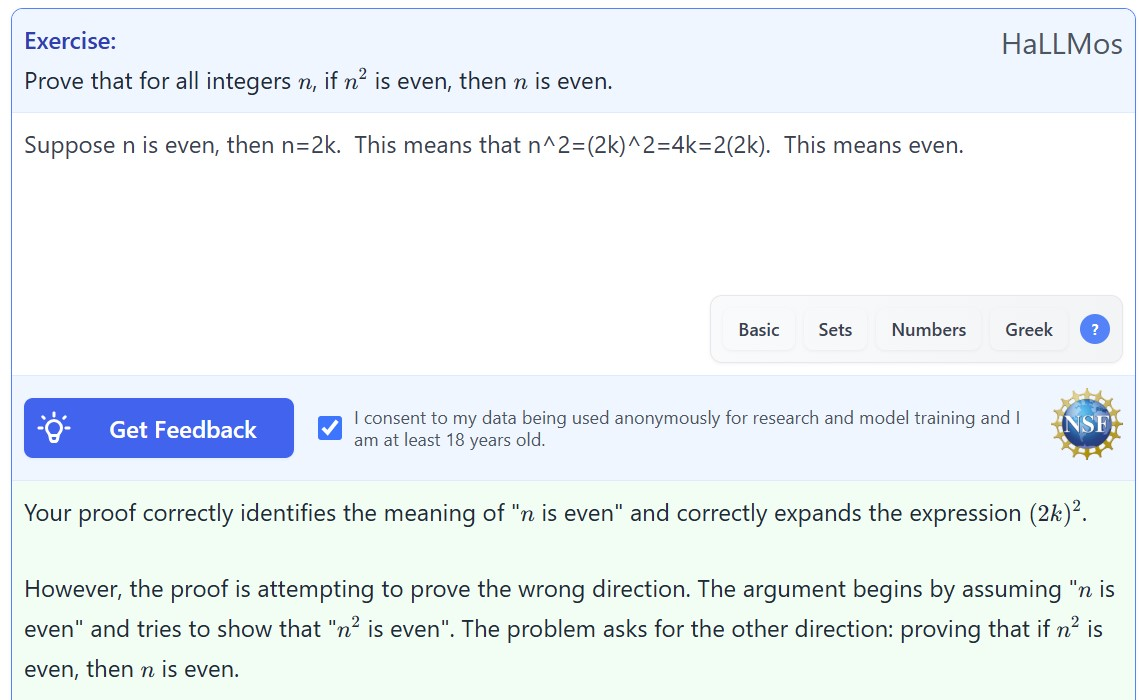
\includegraphics[width=.7\textwidth]{hallmos.jpg}
  \label{F:hallmos}
\end{figure}
This gives us a road-map for providing other sorts of AI interfaces for students. In particular, we would like to build an ``ask me another'' type button where AI asks the student another problem like the one the student is on.

\section*{(ii) AI for Authors}
% AI-supported content development, accessibility improvement, learning
% pathways, efficient updates; tutoring, advising, pathway navigation.
Ximera code was part of the training of AI. \textbf{As a consequence AI are able to produce working Ximera code from simple prompts.} An author can literally describe an activity in broad terms, and AI will write correct code. 

But prompts aren't even needed. In Phase I we performed a proof-of-concept: Sketching ideas on paper and have AI create an Ximera activity.  Figure \ref{F:lineActGPT} shows the snapshot, the prompt, the AI output, and the deployed activity. Note that the prompt requests that the LLM not only produce a Ximera class document, implying that there will be answer boxes for students to fill in, but also generate an additional similar problem.  The code generated by ChatGPT includes the author's original problem and an additional problem, all formatted for Ximera interactivity.
\begin{figure}[h]
  \centering
  \caption{ChatGPT workflow for generating a Ximera activity from a hand-sketch.}
  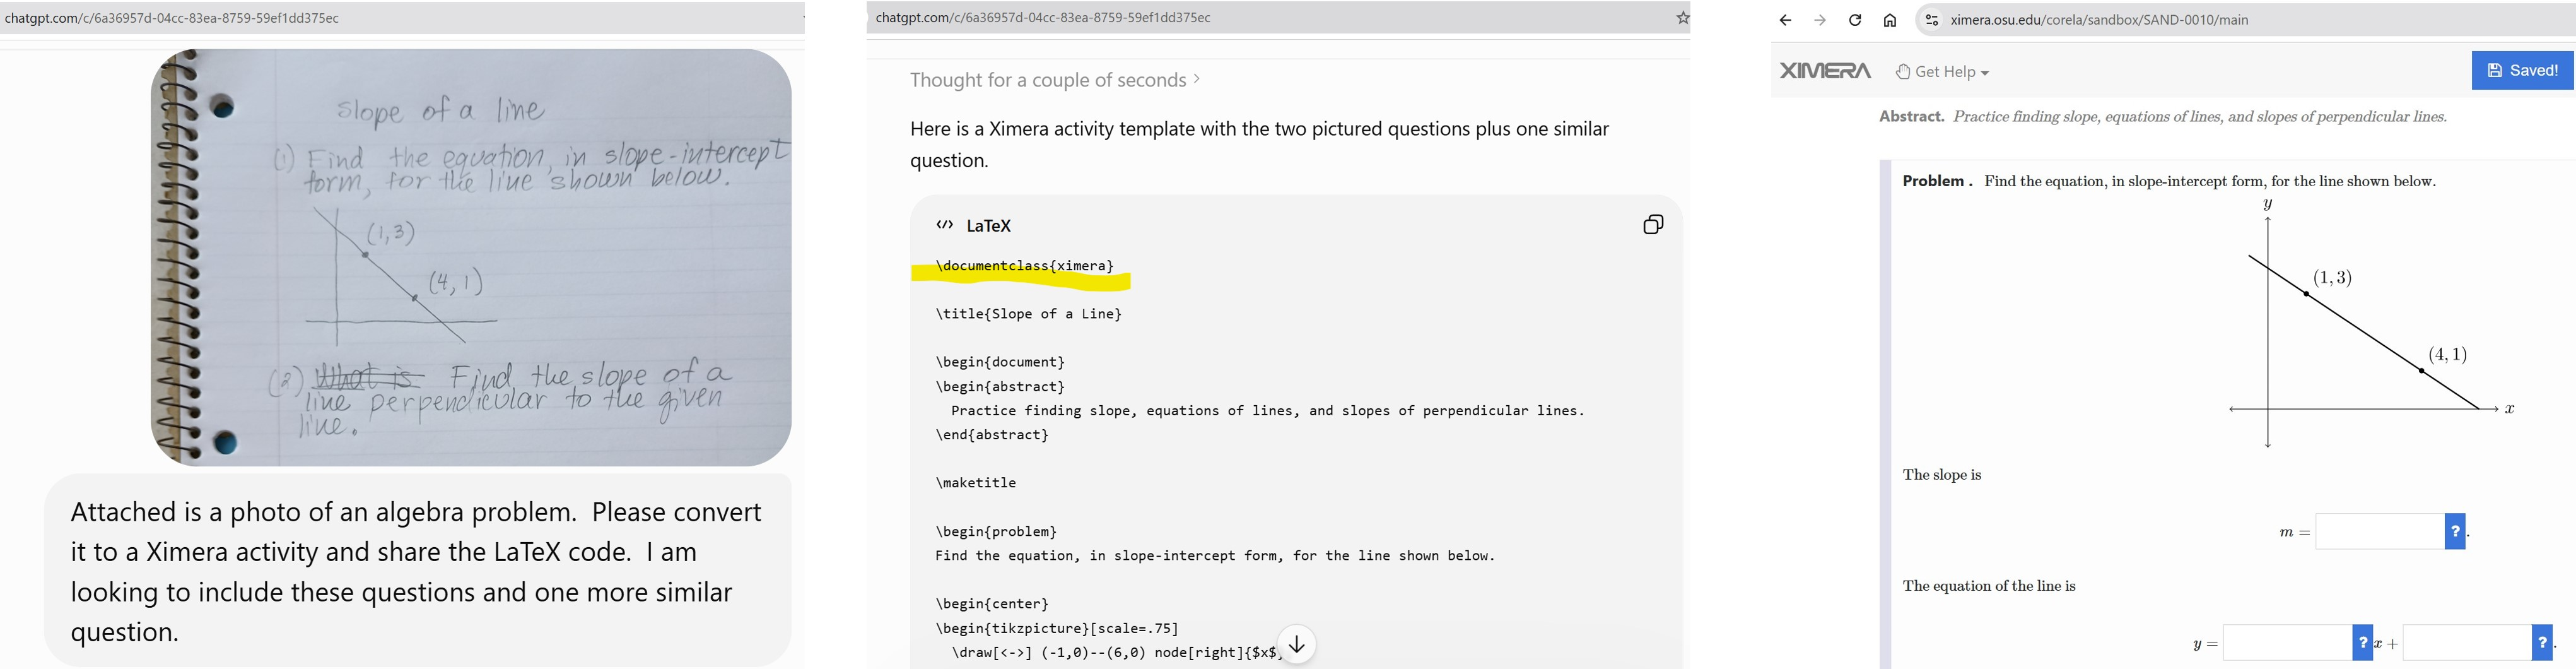
\includegraphics[width=.8\textwidth]{lineActivity.jpg}
  \label{F:lineActGPT}
\end{figure}
Some authors may wish to embed Javascript into their work for more sophisticated interactivity.  Figure \ref{F:parabola} captures the interaction with Claude by a user who is proficient in \LaTeX\ but has never written Javascript.  The third panel in the figure shows an embedded Ximera interactive produced using Javascript generated by Claude.

\begin{figure}[h]
  \centering
  \caption{Claude workflow for generating embeddable Javascript.}
  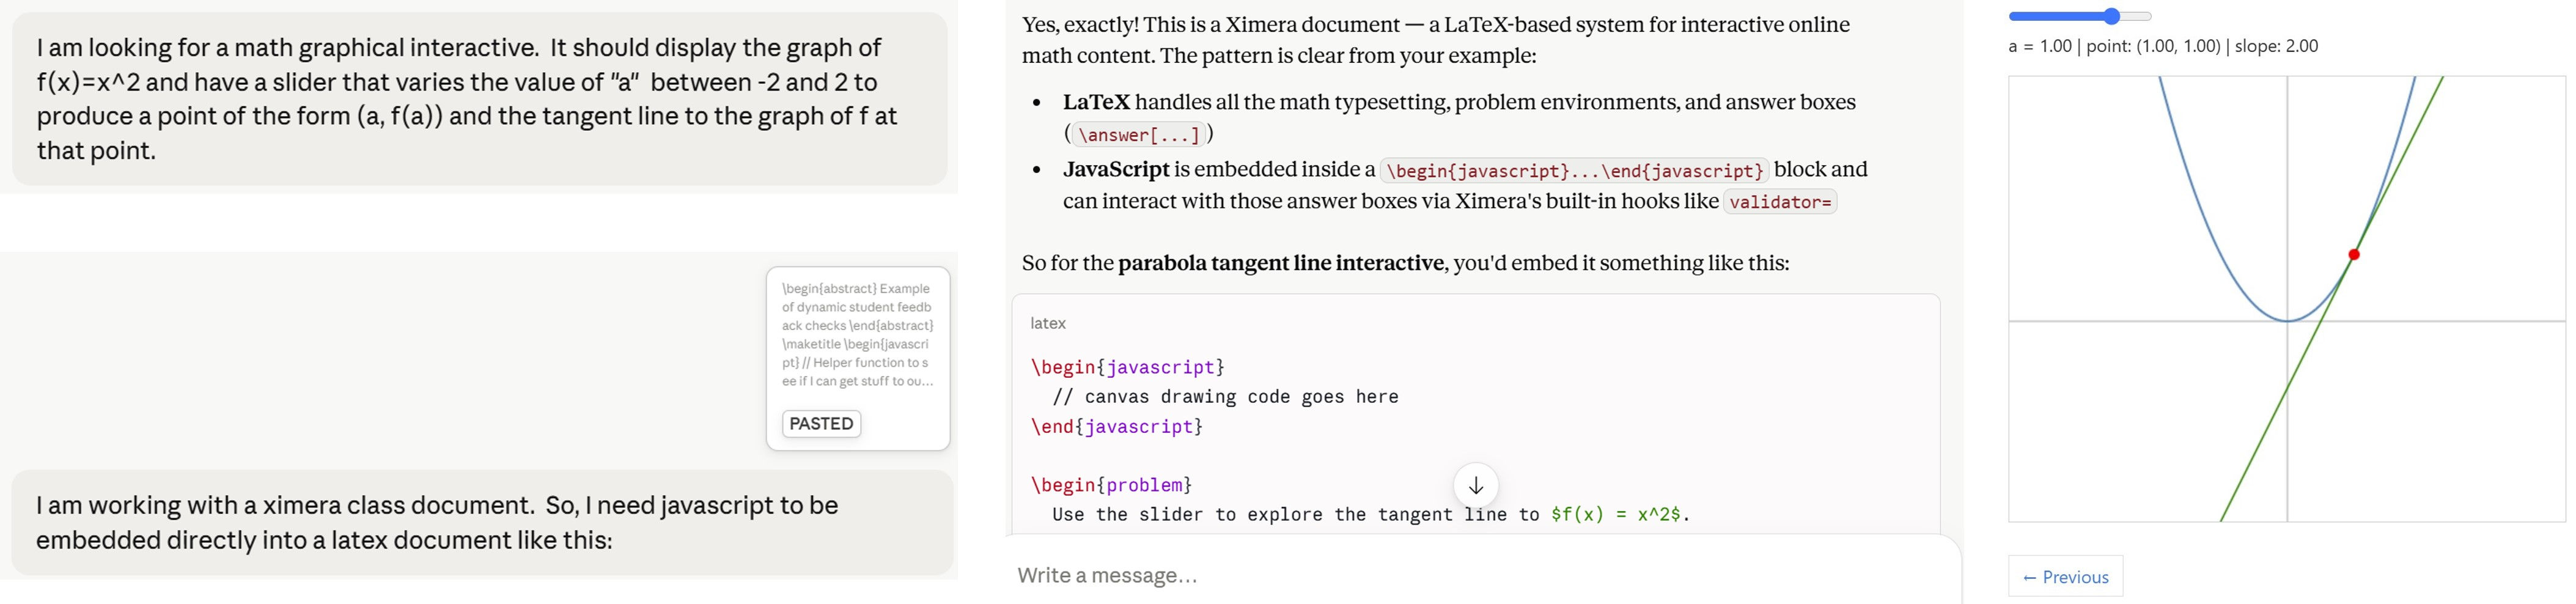
\includegraphics[width=1\textwidth]{parabolaClaude.jpg}
  \label{F:parabola}
\end{figure}

\section*{(ii) AI for Instructors}

Modulus will be recording data on how students use Ximera activities. We will use AI to create data-dashboards that will provide numerous distinct visualizations of the data.



it is important to support authors in their use of AI.  Human develpment of pedagogy and human responsiveness to student needs remains a priority.  We will support authors in their use of AI by connecting them to other Ximera authors with extensive AI experience through the Modulus Atlas program.  We will also incorporate AI training and brainstorming sessions into the annual Ximera Workshops, starting with Ximera Workship 2027.
\end{document}
